\section{Экспериментальные результаты}

\subsection{Методика тестирования}

Для сравнения алгоритмов были проведены замеры времени выполнения на массивах разного размера. Тестирование выполнялось на случайных массивах целых чисел. Каждый эксперимент повторялся 5 раз, в таблице приведены средние значения.

Размер массива \texttt{n} изменялся от 1000 до 100000 элементов.

Характеристики тестовой среды:
\begin{itemize}
    \item Процессор: Intel Core \texttt{i5-1135G7};
    \item Оперативная память: 16 ГБ;
    \item Операционная система: Windows \texttt{11};
    \item Компилятор: GCC \texttt{11.2.0}.
\end{itemize}

\subsection{Результаты замеров}

В табл.~\ref{tab:time} представлены результаты измерения времени выполнения (в миллисекундах) для массивов различного размера \texttt{n}.

\begin{table}[H]
\centering
\caption{Сравнение времени выполнения алгоритмов}
\label{tab:time}
\begin{tabular}{|c|c|c|}
\hline
\textbf{Размер массива (\texttt{n})} & \textbf{Пузырьковая (мс)} & \textbf{Быстрая (мс)} \\
\hline
1000 & 2.34 & 0.12 \\
\hline
5000 & 45.67 & 0.78 \\
\hline
10000 & 187.23 & 1.65 \\
\hline
50000 & 4689.45 & 9.34 \\
\hline
100000 & 18765.32 & 21.56 \\
\hline
\end{tabular}
\end{table}

\subsection{Анализ результатов}

На рис.~\ref{fig:plot} представлен график зависимости времени выполнения от размера массива \texttt{n}.

\begin{figure}[H]
\centering
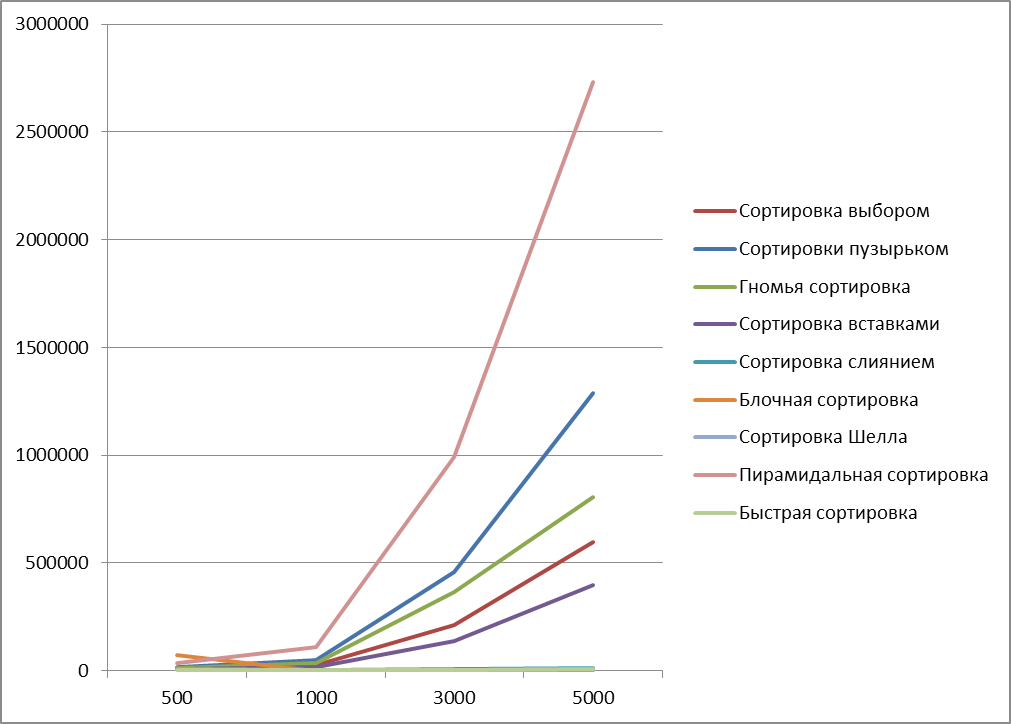
\includegraphics[width=0.8\textwidth]{images/plot.png}
\caption{Зависимость времени выполнения от размера массива \texttt{n}}
\label{fig:plot}
\end{figure}

Как видно из графика, время выполнения пузырьковой сортировки растёт квадратично (\texttt{O(n\textsuperscript{2})}), что делает её непригодной для обработки больших объёмов данных. Для массива из \texttt{n = 100000} элементов она выполняется почти 19 секунд.

Быстрая сортировка демонстрирует линейно-логарифмический рост (\texttt{O(n log n)}). Даже на массиве из \texttt{n = 100000} элементов она выполняется менее 0.1 секунды, что подтверждает её эффективность на практике.

Полученные результаты подтверждают теоретические оценки, приведённые в литературе \cite{knuth1998art, hoare1962quicksort}.